\documentclass{beamer}
\usepackage[utf8]{inputenc}
%\usepackage{multimedia}
\usepackage{tikz}
\usepackage{wasysym}
\setbeamertemplate{itemize item}{\textbullet}	% Itemize dot symbol

\begin{document}

\title{Virtual Theremin}
\subtitle{UIE Project 2015}
\author{A. Alavi, P. Roos, A. Theler}
\date{\today} 

% N e w  F r a m e
\frame{\titlepage} 

% N e w  F r a m e
\frame{
    \frametitle{The Theremin}
    \begin{figure}[p]
        \centering
        \includegraphics[height= 0.5\textwidth]{moogtheremin.jpg}
    \end{figure}
}


% N e w  F r a m e
%\frame{
%    \frametitle{The Theremin}
%    \movie[width=9.6cm, height=7.2cm, autostart]{}{LeonThereminPlayingHisOwnInstrument.mp4}
%}

% N e w  F r a m e
\frame{
    \frametitle{Features}
    For each hand, we extracted the following:
    \itemize{
        \item Palm position ($x,y,z$)
        \item Pinch gesture ($p_0, p_1, p_2, p_3$)
        \item Open/closed hand ($\alpha\in\left[0\ldots1\right]$)
    }
}

% N e w  F r a m e
\frame{
    \frametitle{Pinch Gestures}
    TODO: How it's done
}

% N e w  F r a m e
\frame{
    \frametitle{Open / Closed Hand}
    TODO: How it's done
}

% N e w  F r a m e
\frame{
    \frametitle{The Basic Theremin}

    \vspace{5mm}

    \itemize{
        \item \texttt{leftHand.y} $\to$ Amplitude/Volume
        \item \texttt{rightHand.z} $\to$ frequency
    }

    \vspace{5mm}
    
    $\to$ A playable instrument.


}

% N e w  F r a m e
\frame{
    \frametitle{Findings}
    \itemize{
        \item Precision of Leap Sensor is limited. E.g. it's not possible to accurately play
            a vibrato.
        \item Linear frequency mapping is easier to play.
        \item Leap has difficulties with tracking fingers under the hand palm.
    }
}

% N e w  F r a m e
\frame{
    \frametitle{Improvements Of The Instrument}
    For the right hand:
    \begin{itemize}
        \item Pinch gestures ($p_0, p_1, p_2, p_3$) control different
            waveforms (sinus, triangle, sawtooth and square).
        \item Open/closed hand ($\alpha$) controlls the intensity of a vibrato.
    \end{itemize}

    \vspace{5mm}

    For the left hand:
    \begin{itemize}
        \item Pinch gestures activate frequency discretization (playing aid).
        \item Open/closed hand controls the intensity of a tremolo effect
            (Amplitude Modulation).
    \end{itemize}
}

% N e w  F r a m e
\frame{
    \frametitle{Frequency Discretization - Music Scale}
    Rounding frequency to a musical scale (chromatic, diatonic like major or
    minor, pentatonic).

    \vspace{5mm}

    \begin{center}
    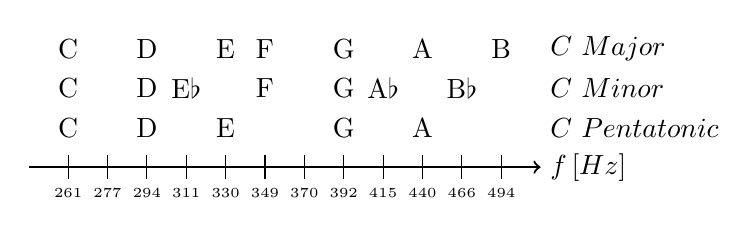
\begin{tikzpicture}[scale=0.5]
        \draw [thick, ->] (-1, 0) -- (12, 0);
        \node [right] at (12, 0) {$f\left[Hz\right]$};

        \foreach \i in {0, ..., 11}{
            \draw (\i, -0.3) -- (\i, 0.3);
        }

        \node [below] at (0, -0.3) {\tiny{261}};
        \node [below] at (1, -0.3) {\tiny{277}};
        \node [below] at (2, -0.3) {\tiny{294}};
        \node [below] at (3, -0.3) {\tiny{311}};
        \node [below] at (4, -0.3) {\tiny{330}};
        \node [below] at (5, -0.3) {\tiny{349}};
        \node [below] at (6, -0.3) {\tiny{370}};
        \node [below] at (7, -0.3) {\tiny{392}};
        \node [below] at (8, -0.3) {\tiny{415}};
        \node [below] at (9, -0.3) {\tiny{440}};
        \node [below] at (10, -0.3) {\tiny{466}};
        \node [below] at (11, -0.3) {\tiny{494}};

        \node at (0, 3) {C};
        \node at (2, 3) {D};
        \node at (4, 3) {E};
        \node at (5, 3) {F};
        \node at (7, 3) {G};
        \node at (9, 3) {A};
        \node at (11,3) {B};
        \node [right] at (12, 3) {$C\ Major$};
        
        \node at (0, 2) {C};
        \node at (2, 2) {D};
        \node at (3, 2) {E$\flat$};
        \node at (5, 2) {F};
        \node at (7, 2) {G};
        \node at (8, 2) {A$\flat$};
        \node at (10,2) {B$\flat$};
        \node [right] at (12, 2) {$C\ Minor$};

        \node at (0, 1) {C};
        \node at (2, 1) {D};
        \node at (4, 1) {E};
        \node at (7, 1) {G};
        \node at (9, 1) {A};
        \node [right] at (12, 1) {$C\ Pentatonic$};

    \end{tikzpicture}
    \end{center}

    \vspace{5mm}
}

% N e w  F r a m e
\frame{
    \frametitle{}
    Thanks for your attention!
}


\end{document}
